% ============================================================
% PROPOSAL PERMOHONAN WAWANCARA NARASUMBER
% Tim beranggotakan lima peserta - Apple Developer Academy @ BINUS
% Urban Innovation Challenge - Juni 2026
% Kompilasi: pdflatex (Overleaf-ready)
% Catatan: butuh paket pdfpages untuk melampirkan surat keterangan academy
% Aset yang harus diunggah bersama file ini:
%   - surat-keterangan-academy.pdf (No. 1738/PEN-SK/VI/2026)
%   - ttdGading.jpeg, ttdKenrich.jpeg, ttdRauf.png, ttdJatayu.jpeg, ttdGina.jpeg
% ============================================================
\documentclass[11pt,a4paper]{article}

\usepackage[T1]{fontenc}
\usepackage[utf8]{inputenc}
\usepackage[indonesian]{babel}
\usepackage[margin=2.5cm]{geometry}
\usepackage{setspace}
\usepackage{enumitem}
\usepackage{tabularx}
\usepackage{parskip}
\usepackage{graphicx}
\usepackage{pdfpages}
\usepackage[hidelinks]{hyperref}

\setstretch{1.15}
\setlist{nosep, leftmargin=*}

\begin{document}

% ---------- KOP ----------
\begin{center}
  {\Large\bfseries PROPOSAL PERMOHONAN WAWANCARA NARASUMBER}\\[4pt]
  {\normalsize Belajar tentang Pengalaman Berjalan Kaki di Jakarta}\\[2pt]
  {\small Tim beranggotakan lima peserta, Apple Developer Academy @ BINUS}
\end{center}

\vspace{4pt}
\hrule
\vspace{14pt}

\noindent
Kepada Yth.\\
\textbf{Bapak H. Anies Rasyid Baswedan, Ph.D.}\\
\textit{Founder} Karsa City Lab\\
di tempat

\vspace{10pt}
Dengan hormat,

% ---------- 1. LATAR BELAKANG ----------
\section*{1. Latar Belakang}

Kami adalah satu tim kecil beranggotakan lima orang, peserta program \textbf{Apple Developer Academy @ BINUS} (diselenggarakan oleh PT~Panji Edukasi Nusantara bersama Apple dan BINUS). Keseharian kami membangun aplikasi di platform Apple dan bekerja dengan data, dan lewat tantangan ini kami ingin belajar mengubah data warga menjadi solusi yang membantu pejalan kaki. Kami sedang menjalani \textit{Urban Innovation Challenge} dengan tema \textit{Urban Living Experience}. Tantangan yang kami pilih untuk dipelajari:

\begin{center}
  \textit{``Make the walking experience in Jakarta more comfortable''}\\
  (membuat pengalaman berjalan kaki di Jakarta lebih nyaman)
\end{center}

Kami ingin belajar tentang koridor transit Sudirman dan kawasan penyangganya di Jakarta Selatan (Setiabudi--Bendungan Hilir--Senayan--Blok M), khususnya 500 meter terakhir perjalanan pejalan kaki menuju dan dari tulang punggung transit Jakarta. Ketertarikan kami pada topik ini tumbuh dari sesi \textbf{Karsa City Lab dan Urun Daya Kota} yang diselenggarakan di akademi pada 10 Juni 2026, yang menekankan pentingnya partisipasi warga, \textit{spatial justice}, dan pendekatan multidisiplin dalam membangun kota.

Saat menyiapkan kegiatan ini, kami belajar bahwa pada masa kepemimpinan Bapak sebagai Gubernur DKI Jakarta (2017--2022), penataan trotoar menjadi salah satu program strategis daerah: pembangunan dan revitalisasi ratusan kilometer trotoar dari rencana induk sekitar 2.600 km, penerapan konsep \textit{complete street}, prioritas pada pusat kegiatan dan simpul perpindahan antarmoda, serta penataan koridor seperti Sudirman--Thamrin, Cikini, Kemang, dan Kota Tua. Pengalaman dan pertimbangan kebijakan di balik program itu tidak kami temukan di buku atau dokumen mana pun. Hal itulah yang ingin kami pelajari langsung dari Bapak.

\newpage
% ---------- 2. MAKSUD DAN TUJUAN ----------
\section*{2. Maksud dan Tujuan}

Melalui proposal ini, kami memohon kesediaan Bapak untuk berbagi pengalaman dalam sebuah wawancara, karena kami ingin belajar tentang:

\begin{enumerate}[label=\alph*., itemsep=2pt]
  \item \textbf{pertimbangan dan proses pengambilan kebijakan} di balik program penataan fasilitas pejalan kaki DKI Jakarta 2017--2022;
  \item \textbf{pengalaman saat menjalankan program tersebut}: hambatan, resistensi, dan hal yang akan Bapak lakukan berbeda, sebagai konteks bagi persoalan pejalan kaki Jakarta hari ini;
  \item \textbf{pandangan dan arahan Bapak} mengenai peran data warga dan teknologi digital dalam meningkatkan kenyamanan serta keamanan berjalan kaki, sebagai masukan bagi solusi yang sedang kami pelajari dan kembangkan.
\end{enumerate}

% ---------- 3. RUANG LINGKUP ----------
\section*{3. Ruang Lingkup Wawancara}

Wawancara bersifat semi-terstruktur dan mencakup tiga tema: (i)~desain dan prioritas kebijakan pejalan kaki 2017--2022; (ii)~tantangan saat menjalankannya dan pelajaran yang Bapak petik; serta (iii)~masa depan pengalaman berjalan kaki di Jakarta dan peran teknologi. Garis besar pertanyaan kami lampirkan pada \textbf{Lampiran~A} agar Bapak dapat meninjau pokok bahasannya. Kami tidak akan menanyakan hal di luar konteks belajar ini.

% ---------- 4. PELAKSANAAN ----------
\section*{4. Waktu, Tempat, dan Format Pelaksanaan}

\begin{tabularx}{\textwidth}{@{}lX@{}}
  Waktu & Pekan 15--19 Juni 2026, \textit{menyesuaikan jadwal Bapak} \\
  Durasi & 60 menit \\
  Format & Tatap muka di lokasi yang Bapak tentukan, atau daring (Zoom/Google Meet) \\
  Peserta & 5 (lima) anggota tim kami \\
  Koordinasi & Teknis pelaksanaan kami koordinasikan melalui staf/ajudan Bapak \\
\end{tabularx}

% ---------- 5. ETIKA ----------
\section*{5. Etika dan Penggunaan Hasil}

\begin{enumerate}[label=\arabic*., itemsep=2pt]
  \item Hasil wawancara kami gunakan \textbf{hanya untuk belajar dan mengembangkan solusi} di lingkup tim kami berlima, bersifat non-komersial, dan tidak kami gunakan untuk pemberitaan maupun keperluan di luar konteks ini.
  \item Kami merekam audio hanya \textbf{atas izin Bapak}; transkrip dan kutipan dapat kami kirimkan untuk Bapak tinjau sebelum kami gunakan.
  \item Kami akan \textbf{membagikan hasil belajar dan pengamatan lapangan kami} kepada Karsa City Lab bila bermanfaat.
\end{enumerate}

\newpage
% ---------- 6. PENUTUP ----------
\section*{6. Penutup}

Demikian proposal ini kami sampaikan. Kami berharap Bapak berkenan meluangkan waktu di tengah kesibukan untuk berbagi pengalaman dengan kami. Surat keterangan resmi dari Apple Developer Academy @ BINUS, yang memuat nama seluruh anggota tim kami, kami sertakan pada \textbf{Lampiran~B}. Atas perhatian dan kesediaan Bapak, kami mengucapkan terima kasih.

\vspace{14pt}
\noindent Tangerang, 16 Juni 2026\\
Hormat kami,\\
Tim kami berlima

\vspace{14pt}
\noindent\textbf{Narahubung}\\
\begin{tabularx}{\textwidth}{@{}lX@{}}
  Nama & {Gading Aditya Perdana} \\
  Telepon/WA & {+62811920059} \\
  Surel & {gading.perdana@binus.ac.id} \\
  Pendamping akademi & {William Chrisandy}, Apple Developer Academy @ BINUS \\
\end{tabularx}

\vspace{2ex}
\begin{tabularx}{\textwidth}{@{} >{\centering\arraybackslash}X >{\centering\arraybackslash}X @{}}
  % Baris 1: Anggota
  \raisebox{-0.8cm}{\includegraphics[height=3cm]{ttdKenrich.jpeg}} &
  \raisebox{-0.4cm}{\includegraphics[height=2cm]{ttdRauf.png}} \\
  \rule{5.2cm}{0.4pt} & \rule{5.2cm}{0.4pt} \\
  {Kenrich Heavenly Sandria} & {Naufal Ammar Rauf} \\
  Anggota Tim & Anggota Tim \\[1cm]

  % Baris 2: Anggota
  \raisebox{-0.4cm}{\includegraphics[height=2cm]{ttdJatayu.jpeg}} &
  \raisebox{-0.1cm}{\includegraphics[height=2cm]{ttdGina.jpeg}} \\
  \rule{5.2cm}{0.4pt} & \rule{5.2cm}{0.4pt} \\
  {Jatayu Muhammad Wicaksono} & {Sintani Gina Lestari} \\
  Anggota Tim & Anggota Tim \\[1cm]

  % Baris 3: Ketua (Tengah)
  \multicolumn{2}{c}{\raisebox{-0.1cm}{\includegraphics[height=3cm]{ttdGading.jpeg}}} \\
  \multicolumn{2}{c}{\rule{5.2cm}{0.4pt}} \\
  \multicolumn{2}{c}{Gading Aditya Perdana} \\
  \multicolumn{2}{c}{Ketua Tim} \\
\end{tabularx}

% ---------- LAMPIRAN B: SURAT KETERANGAN ACADEMY ----------
% Surat Keterangan No. 1738/PEN-SK/VI/2026 dari Apple Developer Academy @ BINUS
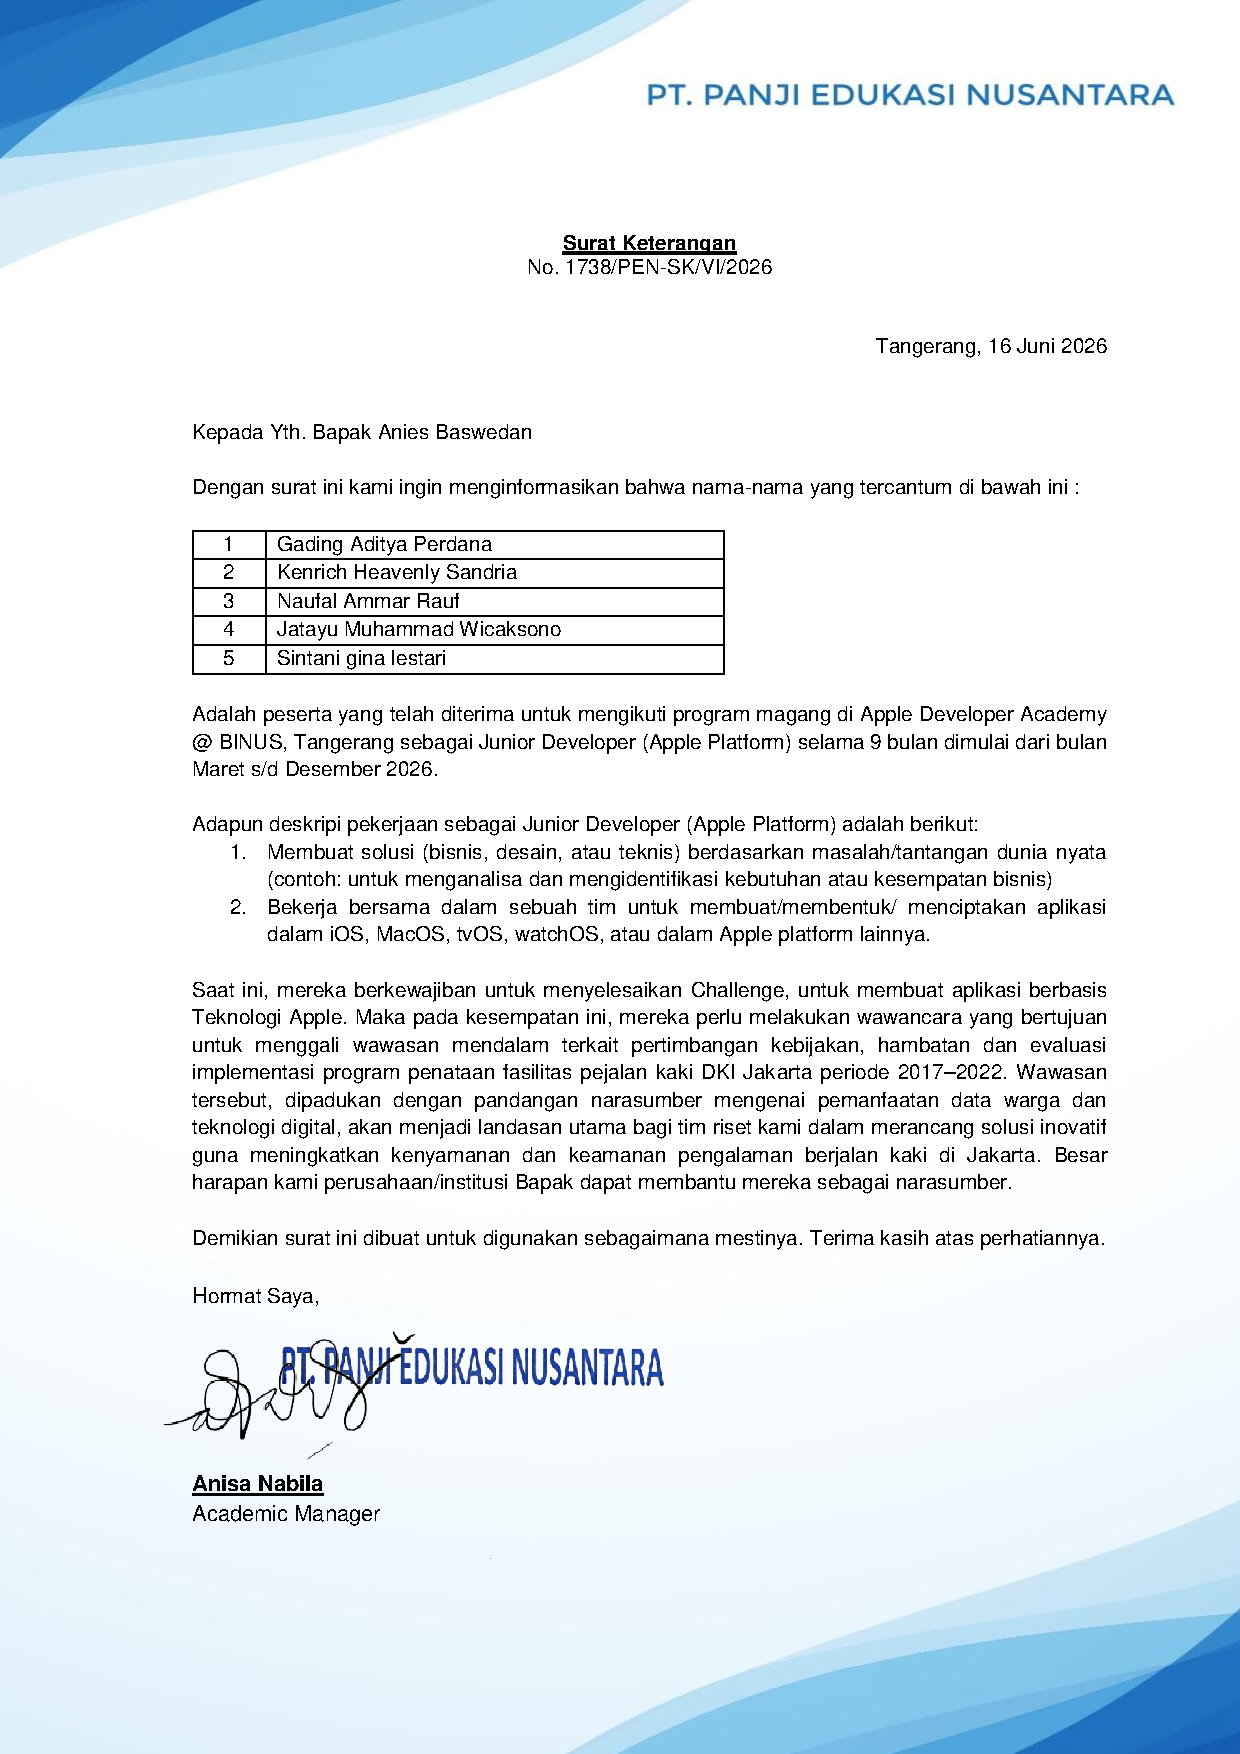
\includepdf[pages=-, pagecommand={\thispagestyle{empty}}]{surat-keterangan-academy.pdf}

\end{document}
